% !TeX program = xelatex
% قالب پایان‌نامه کارشناسی گروه کامپیوتر دانشگاه دامغان
% هماهنگ‌شده با PDF راهنمای نگارش؛ PDF مرجع اولویت دارد.

\documentclass[14pt,a4paper,twoside,openany]{extbook}

\usepackage[
  top=3cm,
  bottom=3cm,
  right=3.75cm,
  left=2.5cm,
  includefoot
]{geometry}
\usepackage{graphicx}
\usepackage{amsmath,amssymb}
\usepackage{booktabs}
\usepackage[table]{xcolor}
\usepackage{longtable}
\usepackage{array}
\usepackage{makecell}
\usepackage{setspace}
\usepackage{titlesec}
\usepackage{caption}
\usepackage{enumitem}
\usepackage{listings}
\usepackage{tikz}
\usepackage{etoolbox}
\usepackage[hidelinks,unicode]{hyperref}
\usepackage{xepersian}
\usetikzlibrary{arrows.meta,positioning,calc,fit,backgrounds}

\newcommand{\UniversityName}{دانشگاه دامغان}
\newcommand{\FacultyName}{دانشکده فنی و مهندسی}
\newcommand{\DegreeName}{پایان‌نامه دوره کارشناسی مهندسی کامپیوتر}
\newcommand{\ThesisTitle}{سایت اشتراک گذاری \lr{API} با پایتون}
\newcommand{\StudentName}{سجاد رضاقلی زاده}
\newcommand{\SupervisorName}{دکتر زهره کریمی}
\newcommand{\ThesisDate}{تیر ۱۴۰۵}

\IfFontExistsTF{B Nazanin}
  {\settextfont[Script=Arabic]{B Nazanin}}
  {\settextfont[Script=Arabic]{Amiri}}

\IfFontExistsTF{Times New Roman}
  {\setlatintextfont[Scale=0.93]{Times New Roman}}
  {\setlatintextfont[Scale=0.93]{Liberation Serif}}

\IfFontExistsTF{Courier New}
  {\setmonofont[Scale=0.90]{Courier New}}
  {\setmonofont[Scale=0.90]{DejaVu Sans Mono}}

\IfFontExistsTF{B Titr}
  {\newfontfamily\titlefont[Script=Arabic,BoldFont={B Titr}]{B Titr}}
  {\newfontfamily\titlefont[Script=Arabic]{Noto Naskh Arabic}}

\renewcommand{\contentsname}{فهرست مطالب}
\renewcommand{\listtablename}{فهرست جدول‌ها}
\renewcommand{\listfigurename}{فهرست نمودارها، عکس‌ها و نقشه‌ها}
\renewcommand{\bibname}{منابع}
\AtBeginDocument{%
  \renewcommand{\bibname}{منابع}%
  \renewcommand{\listfigurename}{فهرست نمودارها، عکس‌ها و نقشه‌ها}%
}

\setstretch{1}
\setlength{\parindent}{0.75cm}
\setlength{\parskip}{0pt}
\setlist{nosep}
\setlist[itemize]{label=-}
\setcounter{secnumdepth}{3}
\setcounter{tocdepth}{3}
\sloppy

\definecolor{damghanNavy}{HTML}{1F3A5F}
\definecolor{damghanTeal}{HTML}{1E6F68}
\definecolor{damghanGold}{HTML}{B7852C}
\definecolor{damghanInk}{HTML}{202A33}
\definecolor{damghanMist}{HTML}{EEF4F6}
\definecolor{tablehead}{HTML}{DCEAF0}
\definecolor{tablestripe}{HTML}{F6F9FA}
\definecolor{tableline}{HTML}{8DA9B8}
\definecolor{codebg}{HTML}{F3F6F7}
\definecolor{codebar}{HTML}{1E6F68}
\arrayrulecolor{tableline}
\setlength{\arrayrulewidth}{0.55pt}
\renewcommand{\arraystretch}{1.32}

\newcommand{\ModernTableStart}{\rowcolors{2}{white}{tablestripe}}
\newcommand{\ModernTableStop}{}
\newcommand{\ChapterRule}{%
  \par\vspace{0.35\baselineskip}%
  {\color{damghanGold}\rule{0.34\textwidth}{0.75pt}}%
  \par\vspace{0.2\baselineskip}%
}
\newcommand{\UniversityLogo}{%
  \IfFileExists{images/university-logo.png}
    {
\includegraphics[width=1.45cm]{images/university-logo.png}}
    {}%
}
\newcommand{\TitlePageFrame}{%
  \begin{tikzpicture}[remember picture,overlay]
    \draw[damghanNavy,line width=0.7pt]
      ([xshift=1.35cm,yshift=-1.35cm]current page.north west)
      rectangle
      ([xshift=-1.35cm,yshift=1.35cm]current page.south east);
    \draw[damghanGold,line width=0.45pt]
      ([xshift=1.55cm,yshift=-1.55cm]current page.north west)
      rectangle
      ([xshift=-1.55cm,yshift=1.55cm]current page.south east);
    \foreach \x/\y in {2.2/4.2,3.6/5.4,5.1/4.7,16.1/22.9,17.4/21.5,15.7/20.8} {
      \fill[damghanTeal,opacity=0.10] ([xshift=\x cm,yshift=\y cm]current page.south west) circle (2pt);
    }
    \draw[damghanTeal,opacity=0.10,line width=0.8pt]
      ([xshift=2.2cm,yshift=4.2cm]current page.south west) --
      ([xshift=3.6cm,yshift=5.4cm]current page.south west) --
      ([xshift=5.1cm,yshift=4.7cm]current page.south west);
    \draw[damghanTeal,opacity=0.10,line width=0.8pt]
      ([xshift=16.1cm,yshift=22.9cm]current page.south west) --
      ([xshift=17.4cm,yshift=21.5cm]current page.south west) --
      ([xshift=15.7cm,yshift=20.8cm]current page.south west);
  \end{tikzpicture}%
}

\makeatletter
\def\ps@thesis{%
  \let\@oddhead\@empty
  \let\@evenhead\@empty
  \def\@oddfoot{\hfil\thepage\hfil}%
  \let\@evenfoot\@oddfoot
}
\let\ps@plain\ps@thesis
\makeatother
\pagestyle{thesis}

\newcommand{\UniversityAbjad}[1]{%
  \ifnum\value{#1}=1 الف\else\abjad{#1}\fi
}

\titleformat{\chapter}[display]
  {\titlefont\bfseries\fontsize{14}{20}\selectfont\centering\color{damghanInk}}
  {{\color{damghanTeal}فصل \thechapter}}
  {0.5\baselineskip}
  {\ChapterRule}
\titlespacing*{\chapter}{0pt}{4\baselineskip}{2\baselineskip}

\titleformat{name=\chapter,numberless}[display]
  {\titlefont\bfseries\fontsize{14}{20}\selectfont\centering\color{damghanInk}}
  {}
  {0pt}
  {\ChapterRule}
\titlespacing*{name=\chapter,numberless}{0pt}{2\baselineskip}{1.5\baselineskip}

\titleformat{\section}
  {\titlefont\bfseries\fontsize{14}{18}\selectfont\color{damghanNavy}}
  {\color{damghanTeal}\lr{\thesection}}
  {0.75em}
  {}

\titleformat{\subsection}
  {\titlefont\bfseries\fontsize{14}{18}\selectfont\color{damghanNavy}}
  {\color{damghanTeal}\lr{\thesubsection}}
  {0.75em}
  {}

\titleformat{\subsubsection}
  {\titlefont\bfseries\fontsize{14}{18}\selectfont\color{damghanNavy}}
  {\color{damghanTeal}\lr{\thesubsubsection}}
  {0.75em}
  {}

\renewcommand{\thesection}{\arabic{section}-\thechapter}
\renewcommand{\thesubsection}{\arabic{subsection}-\arabic{section}-\thechapter}
\renewcommand{\thesubsubsection}{\arabic{subsubsection}-\arabic{subsection}-\arabic{section}-\thechapter}
\renewcommand{\thefigure}{\arabic{figure}-\thechapter}
\renewcommand{\thetable}{\arabic{table}-\thechapter}
\renewcommand{\theequation}{\arabic{equation}-\thechapter}

\DeclareCaptionFont{universitycaption}{\fontsize{12}{15}\selectfont}
\DeclareCaptionLabelFormat{rtl-number}{#1~\lr{#2}}
\DeclareCaptionLabelFormat{appendix-number}{#1~#2}
\captionsetup{
  font=universitycaption,
  labelfont={bf,color=damghanTeal},
  textfont={color=damghanInk},
  labelformat=rtl-number,
  labelsep=space,
  justification=centering,
  singlelinecheck=false
}
\AtBeginEnvironment{table}{\fontsize{12}{15}\selectfont}

\lstset{
  basicstyle=\ttfamily\fontsize{12}{15}\selectfont,
  numbers=left,
  numberstyle=\tiny\color{damghanNavy},
  numbersep=0.4cm,
  xleftmargin=0.6cm,
  backgroundcolor=\color{codebg},
  keywordstyle=\color{damghanNavy}\bfseries,
  commentstyle=\color{damghanTeal},
  stringstyle=\color{damghanGold},
  frame=leftline,
  framerule=1.1pt,
  rulecolor=\color{codebar},
  framesep=5pt,
  breaklines=true,
  columns=fullflexible,
  showstringspaces=false
}

\newcommand{\FrontPage}[2]{%
  \clearpage
  \chapter*{#1}
  \thispagestyle{empty}
  #2
}

\newcommand{\StartAbjadPages}{%
  \clearpage
  \pagenumbering{arabic}
  \renewcommand{\thepage}{\UniversityAbjad{page}}
  \pagestyle{thesis}
}

\newcommand{\StartMainPages}{%
  \clearpage
  \pagenumbering{arabic}
  \pagestyle{thesis}
}

\newcommand{\StartBackMatter}{%
  \clearpage
  \pagenumbering{gobble}
  \pagestyle{empty}
}

\newcommand{\StartAppendices}{%
  \clearpage
  \appendix
  \renewcommand{\thechapter}{\UniversityAbjad{chapter}}
  \renewcommand{\thefigure}{\thechapter-\arabic{figure}}
  \renewcommand{\thetable}{\thechapter-\arabic{table}}
  \renewcommand{\theequation}{\thechapter-\arabic{equation}}
  \captionsetup{labelformat=appendix-number}
  \titleformat{\chapter}[display]
    {\titlefont\bfseries\fontsize{14}{20}\selectfont\centering\color{damghanInk}}
    {{\color{damghanTeal}پیوست \thechapter}}
    {0.5\baselineskip}
    {\ChapterRule}
  \titlespacing*{\chapter}{0pt}{4\baselineskip}{2\baselineskip}
}

\begin{document}

\pagenumbering{gobble}
\pagestyle{empty}

\begin{titlepage}
  \thispagestyle{empty}
  \TitlePageFrame
  \begin{center}
    \vspace*{0.45cm}

    \UniversityLogo\\[0.35cm]

    {\fontsize{14}{20}\selectfont
      \UniversityName\\[0.35cm]
      \FacultyName\\[1.2cm]
      \DegreeName
    }

    \vfill

    {\color{damghanGold}\rule{0.42\textwidth}{0.7pt}}\\[0.55cm]

    {\titlefont\bfseries\fontsize{16}{24}\selectfont
      \ThesisTitle
    }

    \par\vspace{0.55cm}
    {\color{damghanGold}\rule{0.42\textwidth}{0.7pt}}

    \vfill

    {\fontsize{14}{20}\selectfont
      \StudentName
    }

    \vfill

    {\fontsize{14}{20}\selectfont استاد راهنما:}\\[0.3cm]
    {\fontsize{14}{20}\selectfont
      \SupervisorName
    }

    \vfill

    {\fontsize{14}{20}\selectfont \ThesisDate}
    \vspace*{1cm}
  \end{center}
\end{titlepage}

\clearpage
\thispagestyle{empty}
\vspace*{\fill}
\begin{center}
  {\titlefont\bfseries\fontsize{18}{26}\selectfont بسمه‌تعالی}
\end{center}
\vspace*{\fill}

\FrontPage{تشکر و قدردانی}{
از استاد راهنما و همه افرادی که در مسیر انجام این پروژه راهنمایی و حمایت کردند، سپاسگزاری می‌شود.
}

\FrontPage{چکیده}{
این گزارش پروژه \lr{IranAPI Hub} را به عنوان یک پلتفرم فارسی برای اشتراک‌گذاری، جستجو و مصرف \lr{API} بررسی می‌کند. پروژه از بک‌اند \lr{Django REST Framework} و فرانت‌اند \lr{React} استفاده می‌کند و تجربه‌ای شبیه \lr{API Marketplace} ارائه می‌دهد: کاربر می‌تواند کاتالوگ را مرور کند، مستندات را بخواند، وارد حساب خود شود، مصرف و اشتراک را ببیند، \lr{API} منتشر کند و از ابزارهایی مانند \lr{Caller} و \lr{Studio} استفاده کند.

در این گزارش، متن با تمرکز بر تجربه واقعی کاربر، معماری فنی و مسیرهای توسعه آینده نوشته شده است. منابع نظری و فنی از داکیومنت‌های رسمی مانند \lr{Python}، \lr{Django}، \lr{Django REST Framework}، \lr{React}، \lr{Node.js}، \lr{Docker}، \lr{MongoDB}، \lr{OpenAPI} و \lr{RapidAPI} انتخاب شده‌اند. آزمون‌های بک‌اند با دستور \lr{python manage.py test api} اجرا شدند و نتیجه در فصل آزمون آمده است.

\vspace{1cm}
\noindent\textbf{کلیدواژه‌ها:} پلتفرم اشتراک‌گذاری \lr{API}، \lr{Django REST Framework}، \lr{React}، احراز هویت، \lr{OpenAPI}
}

\StartAbjadPages
\tableofcontents

\clearpage
\chapter*{فهرست علائم و نشانه‌ها}
\addcontentsline{toc}{chapter}{فهرست علائم و نشانه‌ها}
\begin{longtable}{>{\raggedleft\arraybackslash}p{3cm} p{9cm}}
\toprule
\rowcolor{tablehead}\textbf{نماد} & \textbf{شرح} \\
\midrule
\ModernTableStart
\lr{API} & رابط برنامه‌نویسی کاربردی \\
\lr{DRF} & \lr{Django REST Framework} \\
\lr{SPA} & برنامه تک‌صفحه‌ای \\
\lr{RTL} & راست‌به‌چپ \\
\lr{ORM} & نگاشت شیء-رابطه \\
\ModernTableStop
\bottomrule
\end{longtable}

\clearpage
\addcontentsline{toc}{chapter}{فهرست جدول‌ها}
\listoftables

\clearpage
\addcontentsline{toc}{chapter}{فهرست نمودارها، عکس‌ها و نقشه‌ها}
\listoffigures

\StartMainPages

\chapter{مقدمه}

این فصل تصویر کلی پروژه را توضیح می‌دهد: چرا چنین سامانه‌ای لازم است، کاربر با آن چه می‌کند، و گزارش از چه زاویه‌ای به پیاده‌سازی نگاه می‌کند. متن تلاش می‌کند فنی باشد، اما خشک و بریده‌بریده نباشد؛ یعنی خواننده ابتدا حس محصول را بگیرد و بعد وارد جزئیات معماری شود.

\section{زمینه پروژه}
\lr{IranAPI Hub} یک پلتفرم فارسی برای معرفی، جستجو، انتشار و مصرف \lr{API} است. فضای پروژه به بازارچه‌های \lr{API} نزدیک است؛ جایی که کاربر می‌تواند سرویس‌ها را ببیند، مستندات را بخواند، پلن‌ها را مقایسه کند و بعد از ورود، مصرف و دسترسی‌های خود را مدیریت کند. این نگاه با مدل رایج \lr{API Hub} و بازارچه‌های \lr{API} هم‌خوان است \cite{rapidapi}.

از نظر فنی، پروژه روی ترکیب \lr{Python}، \lr{Django REST Framework}، \lr{React}، \lr{Vite}، \lr{MongoDB} و \lr{Docker Compose} شکل گرفته است \cite{python,django,drf,react,vite,mongodb,docker}. این ترکیب برای سامانه‌ای مناسب است که هم به یک \lr{API} ساخت‌یافته نیاز دارد و هم به یک رابط کاربری سریع و قابل توسعه.

\section{بیان مسئله}
کاربر چنین سامانه‌ای معمولاً نمی‌خواهد فقط یک فهرست ساده از سرویس‌ها ببیند. او باید بتواند \lr{API}ها را جستجو کند، دسته‌بندی‌ها را بررسی کند، مستندات هر \lr{Endpoint} را بخواند، قیمت یا پلن را بسنجد و بعد از ورود، وضعیت مصرف، کلیدها، اشتراک و سازمان خود را مدیریت کند. توسعه‌دهنده هم نیاز دارد \lr{API} جدید منتشر کند، نمونه درخواست بفرستد و جریان کاری خود را در \lr{Studio} تنظیم کند.

مسئله اصلی، پراکندگی تجربه کاربر است. وقتی مستندات، پرداخت، احراز هویت، مصرف و ابزار تست در چند مسیر جدا باشند، کاربر برای رسیدن به نتیجه باید چند بار زمینه ذهنی خود را عوض کند. این پروژه تلاش می‌کند همین اجزا را در یک تجربه منسجم جمع کند؛ تجربه‌ای که هم برای کاربر عمومی قابل فهم باشد و هم برای توسعه‌دهنده کاربرد عملی داشته باشد.

\section{اهداف}
اهداف اصلی پروژه عبارت‌اند از:
\begin{itemize}
  \item ارائه کاتالوگ \lr{API} با جستجو، دسته‌بندی، امتیاز، پلن و مستندات.
  \item فراهم‌کردن ثبت‌نام، ورود، خروج و نشست کاربر با مدل رایج احراز هویت وب.
  \item نمایش \lr{Dashboard} توسعه‌دهنده شامل پروفایل، \lr{API Key}، مصرف، سازمان و اشتراک.
  \item پشتیبانی از انتشار \lr{API}، اجرای نمونه درخواست در \lr{Caller} و ساخت جریان در \lr{Studio}.
  \item ارائه قرارداد \lr{OpenAPI} برای خوانایی بهتر مسیرها و امکان اتصال ابزارهای دیگر \cite{openapi}.
\end{itemize}

این اهداف فقط به ظاهر سامانه مربوط نیستند. کاتالوگ و مستندات بخش عمومی محصول را می‌سازند؛ ورود، اشتراک و مصرف بخش خصوصی را شکل می‌دهند؛ و \lr{OpenAPI} کمک می‌کند قرارداد سرویس برای انسان و ابزار قابل خواندن باشد.

\section{دامنه و محدودیت‌ها}
دامنه گزارش، نسخه فعلی پروژه و قابلیت‌هایی است که در آن قابل بررسی‌اند: وب‌اپلیکیشن فارسی، \lr{API} بک‌اند، اجرای محلی و جریان‌های اصلی کاربر. اجرای محلی با \lr{Docker Compose} در همین راستا مطرح می‌شود، چون برای بالا آوردن چند سرویس کنار هم طراحی شده است \cite{docker}.

در کنار قابلیت‌ها، چند محدودیت هم باید روشن گفته شود. تنظیمات تولیدی هنوز جای کار دارد، بخشی از رفتارها برای محیط توسعه مناسب‌ترند، پرداخت واقعی و اتصال کامل به سرویس‌های بیرونی نیاز به سخت‌سازی دارد، و آزمون مرورگر باید در چرخه ارزیابی منظم‌تر شود. بنابراین گزارش، پروژه را به عنوان یک نمونه کامل و قابل توسعه بررسی می‌کند، نه یک محصول تولیدی تمام‌شده.

\section{ذی‌نفعان}
ذی‌نفعان اصلی پروژه شامل کاربر مهمان، توسعه‌دهنده احرازشده، مدیر سیستم، ارائه‌دهنده ورود اجتماعی، سرویس مقصد \lr{API} و بازارهای بیرونی مانند \lr{RapidAPI} هستند \cite{rapidapi}. هر کدام از این گروه‌ها انتظار متفاوتی دارند: مهمان به شناخت سریع سرویس نیاز دارد، توسعه‌دهنده به ابزار و داده خصوصی، مدیر به کنترل سامانه، و سرویس‌های بیرونی به قرارداد قابل اعتماد.

\section{سازمان‌دهی گزارش}
فصل دوم فناوری‌ها را معرفی می‌کند. فصل سوم نیازمندی‌ها را دسته‌بندی می‌کند. فصل چهارم معماری را توضیح می‌دهد. فصل پنجم به پیاده‌سازی می‌پردازد. فصل ششم آزمون‌ها را گزارش می‌کند. فصل هفتم نتایج و چالش‌ها را جمع می‌کند و فصل هشتم مسیر ادامه کار را نشان می‌دهد.

\section{جمع‌بندی فصل}
در این فصل مشخص شد که پروژه یک پلتفرم اشتراک‌گذاری و مصرف \lr{API} است؛ نه فقط یک تمرین بک‌اند یا یک رابط کاربری ساده. همین ماهیت دوگانه باعث می‌شود گزارش هم به تجربه کاربر توجه کند و هم به قرارداد فنی بین فرانت‌اند، بک‌اند و داده.

\chapter{فناوری‌ها و پیشینه}

این فصل فناوری‌های اصلی پروژه را معرفی می‌کند و توضیح می‌دهد هر کدام در این سامانه چه نقشی دارند. معیار انتخاب واژه‌ها هم ساده است: هر جا اصطلاح فارسی دقیق و جاافتاده وجود دارد از فارسی استفاده شده، و هر جا ترجمه باعث ابهام می‌شود، اصطلاح اصلی انگلیسی آمده است.

\section{\lr{Python}، \lr{Django} و \lr{Django REST Framework}}
\lr{Python} زبان اصلی بک‌اند است؛ زبانی که به خاطر خوانایی و اکوسیستم گسترده، برای توسعه وب و ساخت سرویس‌های داده‌محور زیاد استفاده می‌شود \cite{python}. روی این زبان، \lr{Django} چارچوب اصلی وب را فراهم می‌کند: تنظیمات، مسیرها، امنیت پایه، مدیریت کاربران، پنل مدیریت و ابزارهای آزمون \cite{django}. 

\lr{Django REST Framework} لایه \lr{API} را روی \lr{Django} کامل‌تر می‌کند. مفاهیمی مثل \lr{View}، \lr{Serializer}، اعتبارسنجی ورودی و پاسخ \lr{JSON} کمک می‌کنند مسیرهای عمومی و خصوصی سامانه با قرارداد منظم‌تری نوشته شوند \cite{drf}. در این پروژه، همین ترکیب برای ساخت کاتالوگ، حساب کاربری، اشتراک، مصرف و ابزارهای توسعه‌دهنده استفاده شده است.

\section{\lr{MongoDB} و مدل داده}
برای داده عملیاتی، پروژه به مدل سندی نزدیک است؛ مدلی که با ساختارهایی مانند کاربر، نشست، \lr{API}، پلن، مصرف و جریان \lr{Studio} راحت‌تر کار می‌کند. \lr{MongoDB} در داکیومنت رسمی خود همین رویکرد سندمحور را برای ذخیره داده‌های انعطاف‌پذیر توضیح می‌دهد \cite{mongodb}. در متن گزارش، وقتی از لایه داده حرف زده می‌شود، منظور همین بخش است که داده‌های محصول را برای مسیرهای بک‌اند آماده می‌کند.

این مدل برای بازارچه \lr{API} منطقی است، چون همه داده‌ها قالب یکسان ندارند. مستندات یک \lr{API}، پلن‌های قیمت‌گذاری، رخدادهای مصرف و جریان‌های \lr{Studio} هر کدام شکل خودشان را دارند. مدل سندی باعث می‌شود این تفاوت‌ها با انعطاف بیشتری نگهداری شوند.

\section{\lr{React}، \lr{TypeScript} و \lr{Vite}}
فرانت‌اند با \lr{React} ساخته شده است؛ کتابخانه‌ای که برای ساخت رابط‌های کاربری مبتنی بر کامپوننت استفاده می‌شود \cite{react}. \lr{TypeScript} هم به کد سمت کاربر نوع‌دهی اضافه می‌کند تا خطاهای ساده زودتر دیده شوند و قرارداد بین بخش‌های مختلف روشن‌تر بماند \cite{typescript}. 

\lr{Vite} ابزار توسعه و \lr{build} فرانت‌اند است. داکیومنت رسمی \lr{Vite} روی سرعت راه‌اندازی و تجربه توسعه سریع تاکید دارد \cite{vite}. این ویژگی برای پروژه‌ای با صفحه‌های مختلف مانند کاتالوگ، جزئیات \lr{API}، \lr{Dashboard}، \lr{Caller} و \lr{Studio} مفید است، چون توسعه رابط کاربری را روان‌تر می‌کند.

\section{\lr{Node.js} و ابزارهای فرانت‌اند}
اکوسیستم فرانت‌اند پروژه روی \lr{Node.js} و ابزارهای بسته‌بندی جاوااسکریپت می‌چرخد. \lr{Node.js} اجرای جاوااسکریپت خارج از مرورگر را فراهم می‌کند و پایه بسیاری از ابزارهای توسعه فرانت‌اند است \cite{nodejs}. کتابخانه‌هایی مثل \lr{TanStack Query}، \lr{Axios} و مجموعه‌های کامپوننتی، کار ارتباط با بک‌اند، مدیریت وضعیت درخواست‌ها و ساخت فرم‌ها و جدول‌ها را ساده‌تر می‌کنند.

در گزارش، نام این ابزارها بدون ترجمه آمده است، چون ترجمه فارسی آن‌ها معمولاً دقیق نیست و ممکن است خواننده را از اصطلاح رایج دور کند.

\section{\lr{Docker Compose} و اجرای محلی}
\lr{Docker Compose} برای تعریف و اجرای چند سرویس کنار هم استفاده می‌شود \cite{docker}. در این پروژه، همین فضا باعث می‌شود بک‌اند و فرانت‌اند در کنار هم بالا بیایند و مسیر ارتباطی مشخصی داشته باشند. این روش برای ارائه، آزمون دستی و توسعه محلی مناسب است، هرچند جای پیکربندی تولیدی را نمی‌گیرد.

\section{\lr{OpenAPI} و \lr{RapidAPI}}
\lr{OpenAPI} برای توصیف قرارداد \lr{API} به‌کار می‌رود؛ یعنی مسیرها، ورودی‌ها، خروجی‌ها و پاسخ‌ها را به شکلی می‌نویسد که هم انسان و هم ابزار بتوانند آن را بخوانند \cite{openapi}. \lr{RapidAPI} نیز نمونه شناخته‌شده‌ای از فضای بازارچه \lr{API} است و برای فهم تجربه کاربر در کشف و مصرف \lr{API} مرجع خوبی به شمار می‌آید \cite{rapidapi}.

\section{جمع‌بندی فصل}
پشته فنی پروژه با ماهیت آن هماهنگ است: \lr{Django REST Framework} برای ساخت \lr{API}، \lr{React} برای تجربه کاربری، \lr{MongoDB} برای داده‌های سندی، \lr{Docker Compose} برای اجرای محلی، و \lr{OpenAPI} برای خوانایی قرارداد سرویس. این ترکیب، فضای گزارش را هم به سمت یک محصول واقعی اشتراک‌گذاری \lr{API} می‌برد.

\chapter{تحلیل نیازمندی‌ها}

این فصل نیازمندی‌های پروژه را از زاویه تجربه کاربر و رفتار سامانه دسته‌بندی می‌کند. هدف این نیست که فقط یک فهرست خشک ارائه شود؛ هر نیازمندی باید نشان دهد کاربر چه انتظاری دارد و سامانه برای پاسخ به آن چه رفتاری باید داشته باشد.

\section{نقش‌های کاربری}
سه نقش اصلی در پروژه دیده می‌شود: مهمان، توسعه‌دهنده احرازشده و مدیر سیستم. مهمان بخش عمومی کاتالوگ را می‌بیند. توسعه‌دهنده بعد از ورود، با \lr{Dashboard}، انتشار \lr{API}، \lr{Caller} و \lr{Studio} کار می‌کند. مدیر سیستم هم مسئول کنترل کلی و نگهداری داده‌هاست.

\begin{figure}[htbp]
  \centering
  \begin{tikzpicture}[
    >=Latex,
    every node/.style={font=\fontsize{12}{14}\selectfont, align=center},
    actor/.style={draw=damghanNavy, very thick, rounded corners=2pt, fill=tablehead, minimum width=2.9cm, minimum height=0.75cm},
    action/.style={draw=tableline, thick, rounded corners=2pt, fill=white, minimum width=3.1cm, minimum height=0.72cm},
    flow/.style={-{Latex[length=2.2mm]}, thick, color=damghanTeal}
  ]
    \node[actor] (guest) at (4,2.2) {مهمان};
    \node[actor] (developer) at (4,0) {توسعه‌دهنده};
    \node[actor] (admin) at (4,-2.2) {مدیر سیستم};

    \node[action] (browse) at (-2.2,2.8) {مرور کاتالوگ};
    \node[action] (docs) at (-2.2,1.6) {مشاهده مستندات};
    \node[action] (account) at (-2.2,0.6) {حساب و سازمان};
    \node[action] (release) at (-2.2,-0.6) {انتشار \lr{API}};
    \node[action] (studio) at (-2.2,-1.8) {\lr{Caller} و \lr{Studio}};
    \node[action] (panel) at (-2.2,-3.0) {پنل مدیریت};

    \draw[flow] (guest.west) -- (browse.east);
    \draw[flow] (guest.west) -- (docs.east);
    \draw[flow] (developer.west) -- (account.east);
    \draw[flow] (developer.west) -- (release.east);
    \draw[flow] (developer.west) -- (studio.east);
    \draw[flow] (admin.west) -- (panel.east);
  \end{tikzpicture}
  \caption{نمای نقش‌ها و جریان‌های اصلی پروژه}
  \label{fig:roles}
\end{figure}

نقش مهمان بدون ورود می‌تواند بخش عمومی بازارچه را ببیند؛ این بخش برای جذب کاربر و معرفی \lr{API}ها ضروری است. نقش توسعه‌دهنده پس از احراز هویت به امکاناتی دسترسی دارد که با داده خصوصی کاربر ارتباط دارند، مانند کلید \lr{API}، سازمان، اشتراک، مصرف، انتشار و ابزارهای آزمایشی. نقش مدیر سیستم بیشتر به نگهداری داده و پشتیبانی از مسیرهای مدیریتی مربوط می‌شود و از نظر سطح دسترسی از دو نقش دیگر حساس‌تر است.

\section{نیازمندی‌های عملکردی و غیرفعال}
جدول \ref{tab:reqs} نیازمندی‌ها را در دو گروه اصلی نشان می‌دهد. نیازمندی‌های عملکردی به کارهایی مربوط‌اند که کاربر مستقیماً می‌بیند؛ مثل جستجوی \lr{API}، ورود، انتشار یا مشاهده مصرف. نیازمندی‌های امنیتی و اجرایی کیفیت همین رفتارها را حفظ می‌کنند؛ مثل پنهان‌کردن کلیدها، پاسخ خطای قابل فهم و اجرای محلی با \lr{Docker Compose}.

\begin{longtable}{p{1.35cm} p{5.25cm} p{1.75cm} p{1.35cm} p{1.85cm}}
\caption{نیازمندی‌های اصلی پروژه}\label{tab:reqs}\\
\toprule
\rowcolor{tablehead}\textbf{شناسه} & \textbf{نیازمندی} & \textbf{نوع} & \textbf{اولویت} & \textbf{وضعیت} \\
\midrule
\endfirsthead
\toprule
\rowcolor{tablehead}\textbf{شناسه} & \textbf{نیازمندی} & \textbf{نوع} & \textbf{اولویت} & \textbf{وضعیت} \\
\midrule
\endhead
\ModernTableStart
\lr{R1} & نمایش فهرست \lr{API}ها با صفحه‌بندی، جستجو، دسته‌بندی و مرتب‌سازی & عملکردی & زیاد & انجام‌شده \\
\lr{R2} & نمایش جزئیات، پلن‌ها، مستندات، \lr{endpoint}ها و \lr{API}های مشابه & عملکردی & زیاد & انجام‌شده \\
\lr{R3} & ثبت‌نام، ورود، نشست، خروج و کشف ارائه‌دهندگان ورود اجتماعی & عملکردی & زیاد & انجام‌شده \\
\lr{R4} & مدیریت کاربر، پروفایل، سازمان، اشتراک، پرداخت دستی و مصرف & عملکردی & زیاد & انجام‌شده \\
\lr{R5} & انتشار \lr{API} توسط کاربر احرازشده & عملکردی & متوسط & انجام‌شده \\
\lr{R6} & اجرای درخواست نمونه در \lr{Caller} و ثبت مصرف & عملکردی & متوسط & انجام‌شده \\
\lr{R7} & استقرار جریان \lr{Studio} و ثبت مصرف & عملکردی & متوسط & انجام‌شده \\
\lr{R8} & بازگشت خطای یکنواخت برای اعتبارسنجی و دسترسی & غیرفعال & زیاد & انجام‌شده \\
\lr{R9} & پنهان‌سازی کلیدها و توکن‌ها در پاسخ‌ها و لاگ‌ها & امنیتی & زیاد & انجام‌شده \\
\lr{R10} & اجرای محلی دو سرویس با \lr{Docker Compose} & استقرار & متوسط & مستند \\
\ModernTableStop
\bottomrule
\end{longtable}

اولویت زیاد برای نیازهایی در نظر گرفته شده که نبود آن‌ها باعث از کار افتادن هسته محصول می‌شود؛ مانند کاتالوگ، احراز هویت، حساب کاربری و امنیت داده حساس. اولویت متوسط برای قابلیت‌هایی است که ارزش محصول را کامل‌تر می‌کنند، اما می‌توانند در نسخه‌های بعدی نیز تکامل پیدا کنند؛ مانند \lr{Studio}، \lr{Caller} و اجرای محلی.

\section{ورودی‌ها، خروجی‌ها و اعتبارسنجی}
ورودی‌های اصلی شامل مشخصات حساب، پروفایل، شناسه یا نامک \lr{API}، فیلترهای جستجو، امتیاز، داده انتشار \lr{API}، شناسه پلن اشتراک و گره‌های \lr{Studio} است. در معماری مبتنی بر \lr{Django REST Framework}، معمولاً \lr{Serializer} مسئول کنترل و تبدیل همین داده‌هاست \cite{drf}.

خروجی‌های اصلی سامانه در قالب \lr{JSON} بازگردانده می‌شوند و برای مصرف فرانت‌اند طراحی شده‌اند. پاسخ‌های عمومی معمولاً شامل داده کاتالوگ، مستندات، پلن‌ها و وضعیت سلامت هستند. پاسخ‌های خصوصی شامل داده‌هایی مانند پروفایل، سازمان‌ها، کلید پنهان‌شده، اشتراک و تاریخچه مصرف هستند. جداسازی این دو دسته خروجی اهمیت دارد، زیرا داده عمومی برای همه کاربران قابل نمایش است، اما داده خصوصی باید فقط بعد از احراز هویت برگردد.

اعتبارسنجی در این پروژه دو نقش دارد: نخست جلوگیری از ذخیره داده ناقص یا نامعتبر، و دوم تبدیل خطا به پاسخ قابل فهم برای \lr{Client}. برای نمونه، هنگام ثبت امتیاز باید مقدار امتیاز معتبر باشد، هنگام انتشار \lr{API} فیلدهای اصلی باید حاضر باشند و هنگام اجرای \lr{Studio} ساختار گره‌ها باید قابل پردازش باشد.

\section{امنیت}
احراز هویت باید به شکلی باشد که کاربر بعد از ورود بتواند به بخش‌های خصوصی دسترسی داشته باشد، اما داده حساس او در پاسخ‌ها آشکار نشود. در پروژه‌هایی که با \lr{API Key}، توکن و کوکی کار می‌کنند، این موضوع فقط یک انتخاب ظاهری نیست؛ بخشی از امنیت اصلی محصول است \cite{django,drf}.

از دید نیازمندی، امنیت فقط ورود کاربر نیست؛ بلکه کنترل دسترسی، نگهداری نشست، جلوگیری از افشای رازها و محدودکردن خروجی‌های حساس را نیز شامل می‌شود. آزمون‌های موجود نشان می‌دهند که پنهان‌سازی داده حساس در خروجی‌ها بررسی شده است. با این حال، برای محیط تولید باید رازهای پیکربندی از فایل تنظیمات خارج شوند و سیاست‌های سخت‌گیرانه‌تری برای کوکی، دامنه مجاز و خطاهای عملیاتی اعمال شود.

\section{جمع‌بندی فصل}
نیازهای پروژه حول کشف عمومی \lr{API}، فضای کاری توسعه‌دهنده، مدیریت حساب و اشتراک، و امنیت نشست شکل گرفته‌اند. این نیازمندی‌ها مبنای فصل معماری هستند؛ چون لایه‌های سامانه باید همین نقش‌ها، جریان‌ها و محدودیت‌های امنیتی را پشتیبانی کنند.

\chapter{معماری و طراحی}

این فصل معماری سامانه را با زبان ساده توضیح می‌دهد. مسیر کلی چنین است: کاربر از رابط \lr{React} شروع می‌کند، درخواست به بک‌اند \lr{Django REST Framework} می‌رسد، داده اعتبارسنجی می‌شود و در نهایت لایه داده نتیجه را آماده می‌کند.

\section{نمای کلی}
معماری پروژه سه لایه اصلی دارد: رابط کاربری \lr{React}، بک‌اند \lr{Django REST Framework} و لایه داده. این مدل با الگوی رایج وب‌اپلیکیشن‌های مدرن هماهنگ است؛ فرانت‌اند تجربه کاربر را می‌سازد، بک‌اند قرارداد \lr{API} را مدیریت می‌کند و لایه داده مسئول نگهداری اطلاعات محصول است \cite{react,drf,mongodb}.

این طراحی باعث می‌شود کاربر نهایی بیشتر با یک برنامه تک‌صفحه‌ای روبه‌رو باشد، در حالی که عملیات داده از طریق \lr{API} نسخه‌دار انجام می‌شود. نسخه‌دار بودن مسیرها برای نگهداری آینده مهم است، زیرا امکان تغییر یا اضافه‌کردن قراردادهای جدید را بدون شکستن \lr{Client}های قدیمی فراهم می‌کند. همچنین نمایش پوسته \lr{SPA} برای مسیرهای ناشناخته فرانت‌اند، با الگوی مسیریابی سمت \lr{Client} سازگار است.

\section{نمودار معماری}
\begin{figure}[htbp]
  \centering
  \begin{latin}
  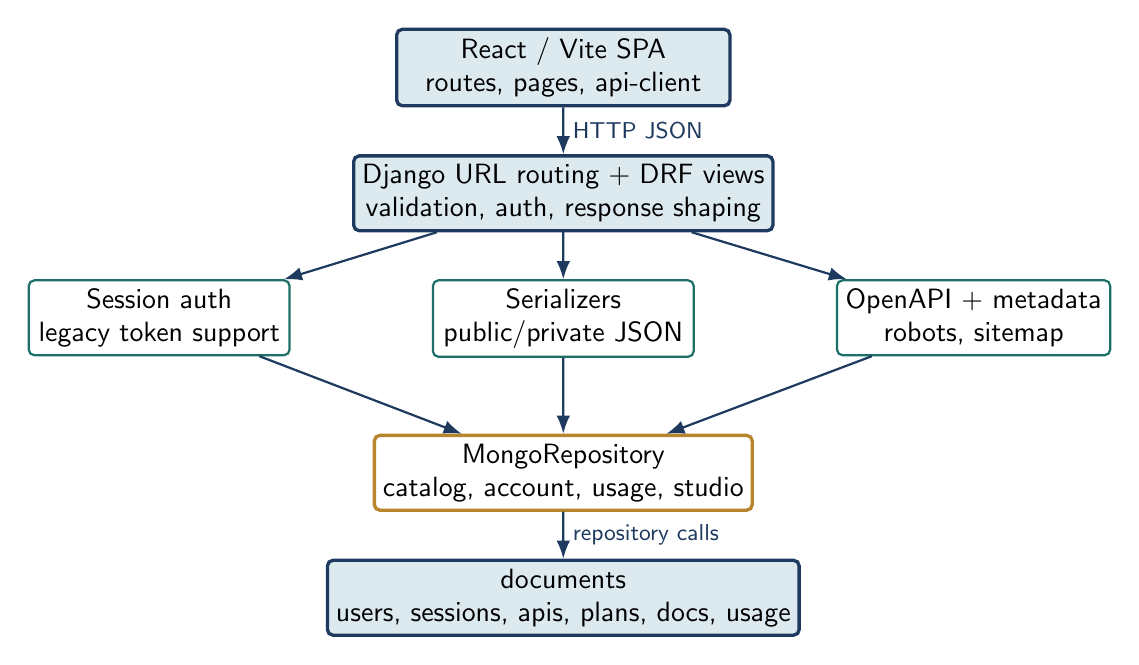
\begin{tikzpicture}[
    scale=0.92,
    transform shape,
    node distance=0.65cm and 0.85cm,
    every node/.style={font=\sffamily\fontsize{10.5}{13}\selectfont, align=center},
    layer/.style={draw=damghanNavy, very thick, rounded corners=2pt, fill=tablehead, minimum width=4.6cm, minimum height=0.85cm},
    service/.style={draw=damghanTeal, thick, rounded corners=2pt, fill=white, minimum width=3.6cm, minimum height=0.75cm},
    store/.style={draw=damghanGold, very thick, rounded corners=2pt, fill=white, minimum width=4.8cm, minimum height=0.85cm},
    flow/.style={-{Latex[length=2.3mm]}, thick, color=damghanNavy}
  ]
    \node[layer] (spa) {React / Vite SPA\\routes, pages, api-client};
    \node[layer, below=of spa] (api) {Django URL routing + DRF views\\validation, auth, response shaping};
    \node[service, below left=of api] (auth) {Session auth\\legacy token support};
    \node[service, below=of api] (serializers) {Serializers\\public/private JSON};
    \node[service, below right=of api] (schemas) {OpenAPI + metadata\\robots, sitemap};
    \node[store, below=1.05cm of serializers] (repo) {MongoRepository\\catalog, account, usage, studio};
    \node[layer, below=of repo] (data) {documents\\users, sessions, apis, plans, docs, usage};

    \draw[flow] (spa) -- node[right, font=\sffamily\fontsize{9}{11}\selectfont] {HTTP JSON} (api);
    \draw[flow] (api) -- (auth);
    \draw[flow] (api) -- (serializers);
    \draw[flow] (api) -- (schemas);
    \draw[flow] (auth) -- (repo);
    \draw[flow] (serializers) -- (repo);
    \draw[flow] (schemas) -- (repo);
    \draw[flow] (repo) -- node[right, font=\sffamily\fontsize{9}{11}\selectfont] {repository calls} (data);
  \end{tikzpicture}
  \end{latin}
  \caption{معماری سطح بالای پروژه}
  \label{fig:architecture}
\end{figure}

مطابق شکل \ref{fig:architecture}، فرانت‌اند درخواست‌ها را به \lr{API} بک‌اند می‌فرستد. بک‌اند، ورودی را اعتبارسنجی می‌کند، پاسخ را به قالب \lr{JSON} درمی‌آورد و کار با داده را به لایه \lr{Repository} می‌سپارد.

در این معماری، هر لایه کار خودش را انجام می‌دهد. فرانت‌اند مسئول نمایش، فرم‌ها و حرکت کاربر بین صفحه‌هاست. بک‌اند مسئول احراز هویت، اعتبارسنجی و شکل پاسخ است. \lr{Repository} هم جزئیات ذخیره‌سازی و بازیابی داده را پنهان می‌کند. همین جداسازی باعث می‌شود تغییر در ظاهر کاربر، کل منطق داده را به‌هم نریزد.

\section{مدل داده}
مدل داده پروژه حول چند گروه اصلی می‌چرخد: هویت کاربر، کاتالوگ \lr{API}، دسترسی و مصرف، فضای کاری توسعه‌دهنده و اشتراک. این تقسیم‌بندی با مدل سندی \lr{MongoDB} سازگار است، چون هر گروه می‌تواند ساختار و جزئیات خودش را داشته باشد \cite{mongodb}.

\begin{longtable}{p{4cm} p{8cm}}
\caption{گروه‌های داده اصلی}\label{tab:data-model}\\
\toprule
\rowcolor{tablehead}\textbf{گروه} & \textbf{مجموعه‌ها و مسئولیت} \\
\midrule
\endfirsthead
\toprule
\rowcolor{tablehead}\textbf{گروه} & \textbf{مجموعه‌ها و مسئولیت} \\
\midrule
\endhead
\ModernTableStart
هویت & \lr{users}، \lr{sessions} و \lr{legacy\_tokens} برای کاربر، نشست و توکن سازگار \\
کاتالوگ & \lr{categories}، \lr{apis}، \lr{pricing\_plans}، \lr{documentations}، \lr{api\_endpoints} و \lr{api\_ratings} \\
مصرف & \lr{access\_grants} و \lr{api\_usage} برای مجوز دسترسی و رخدادهای مصرف \\
فضای کاری & \lr{organizations} و \lr{studio\_flows} برای امکانات توسعه‌دهنده \\
اشتراک & \lr{subscription\_plans}، \lr{user\_subscriptions} و \lr{subscription\_checkouts} \\
\ModernTableStop
\bottomrule
\end{longtable}

گروه هویت پایه دسترسی کاربر را می‌سازد و به نشست‌ها و توکن‌های سازگار قدیمی متصل است. گروه کاتالوگ محتوای عمومی بازارچه را نگه می‌دارد؛ یعنی دسته‌ها، خود \lr{API}ها، پلن قیمت‌گذاری، مستندات، نقاط انتهایی و امتیازها. گروه مصرف و اشتراک داده‌هایی را ثبت می‌کند که برای داشبورد، کنترل دسترسی و گزارش استفاده لازم‌اند. گروه فضای کاری نیز قابلیت‌های مخصوص توسعه‌دهنده مانند سازمان و جریان \lr{Studio} را پشتیبانی می‌کند.

\section{مرزهای خارجی}
مرزهای خارجی پروژه شامل ارائه‌دهندگان ورود اجتماعی، سرویس مقصد \lr{API} و بازارهای بیرونی مانند \lr{RapidAPI} است \cite{rapidapi}. این مرزها باید روشن باشند، چون هر کدام سطحی از ریسک و وابستگی بیرونی وارد سامانه می‌کنند.

شناخت مرز خارجی برای تحلیل ریسک مهم است. ورود اجتماعی به پیکربندی ارائه‌دهنده وابسته است و در صورت نبود \lr{auth\_url} نمی‌تواند کامل اجرا شود. \lr{Caller} و \lr{Studio} نیز از نظر محصول به ارتباط با سرویس‌های بیرونی نزدیک هستند، اما در وضعیت فعلی بیشتر برای نمایش جریان و ثبت مصرف استفاده می‌شوند. بنابراین گزارش بین قابلیت پیاده‌سازی‌شده و اتصال تولیدی واقعی تفاوت می‌گذارد.

\section{جمع‌بندی فصل}
معماری پروژه یک \lr{SPA} متصل به \lr{API} بک‌اند است. این طراحی برای نمونه محصول مناسب است و فضای پروژه را به یک پلتفرم واقعی \lr{API} نزدیک می‌کند. برای استفاده تولیدی، تصمیم نهایی درباره پایگاه داده، مدیریت رازها و اتصال‌های بیرونی باید دقیق‌تر شود.

\chapter{پیاده‌سازی}

این فصل پیاده‌سازی را از زاویه رفتار سامانه توضیح می‌دهد. به جای تکیه روی جزئیات داخلی پروژه، مسیر ذهنی کاربر و نقش هر بخش فنی بیان می‌شود؛ چون خواننده گزارش باید بفهمد محصول چگونه کار می‌کند، نه این‌که درگیر نام داخلی فایل‌ها شود.

\section{مسیرهای بک‌اند}
بک‌اند مجموعه‌ای از مسیرهای نسخه‌دار دارد که بخش‌های اصلی محصول را پوشش می‌دهند: سلامت سامانه، قرارداد \lr{OpenAPI}، ثبت‌نام، ورود، خروج، حساب کاربری، پروفایل، \lr{API Key}، سازمان‌ها، اشتراک، مصرف، کاتالوگ، مستندات، \lr{Endpoint}ها، \lr{Caller} و \lr{Studio}. استفاده از مسیرهای نسخه‌دار برای \lr{API} کمک می‌کند توسعه آینده کنترل‌شده‌تر باشد و \lr{Client}ها با تغییرات ناگهانی روبه‌رو نشوند \cite{drf,openapi}.

این مسیرها دو سطح تجربه می‌سازند. سطح اول عمومی است و برای مشاهده کاتالوگ، جزئیات \lr{API} و مستندات استفاده می‌شود. سطح دوم خصوصی است و بعد از ورود کاربر فعال می‌شود؛ مثل \lr{Dashboard}، مصرف، اشتراک، سازمان و انتشار \lr{API}.

\section{لایه \lr{Repository}}
لایه \lr{Repository} منطق کار با داده را متمرکز می‌کند. ساخت کاربر، نگهداری نشست، چرخش \lr{API Key}، خواندن کاتالوگ، ثبت مصرف \lr{Caller} و ذخیره جریان‌های \lr{Studio} از همین مسیر انجام می‌شود. این شیوه باعث می‌شود \lr{View}ها بیش از حد شلوغ نشوند و جزئیات داده در یک لایه مشخص بماند.

در پروژه‌ای شبیه بازارچه \lr{API}، این جداسازی مهم است. داده‌های حساب، کاتالوگ، مستندات، اشتراک و مصرف شکل یکسانی ندارند. وقتی این بخش‌ها پشت یک \lr{Repository} قرار می‌گیرند، تغییر در روش ذخیره‌سازی کمتر به بخش‌های دیگر نشت می‌کند.

\section{\lr{Serializer} و قرارداد پاسخ}
\lr{Serializer}ها نقش مرز امن بین داده داخلی و خروجی قابل نمایش را دارند. داده‌ای که داخل سامانه نگهداری می‌شود، همیشه نباید با همان شکل به کاربر برگردد. برای نمونه، مقدار کامل \lr{API Key} نباید در پاسخ عادی دیده شود و بهتر است فقط نسخه پنهان‌شده آن نمایش داده شود. این رویکرد با نقش \lr{Serializer} در \lr{Django REST Framework} هماهنگ است \cite{drf}.

در بخش انتشار \lr{API} نیز \lr{Serializer} کمک می‌کند داده ورودی قبل از ثبت بررسی شود: نام، آدرس پایه، روش احراز هویت، دسته و توضیح سرویس باید روشن باشند. نتیجه این کار، پاسخ‌هایی است که برای فرانت‌اند قابل پیش‌بینی‌ترند.

\section{فرانت‌اند}
فرانت‌اند تجربه اصلی کاربر را می‌سازد: صفحه مرور \lr{API}ها، جزئیات سرویس، مستندات، قیمت‌گذاری، پرداخت، ورود، ثبت‌نام، \lr{Dashboard}، سازمان‌ها، انتشار، \lr{Caller} و \lr{Studio}. معماری کامپوننتی \lr{React} برای چنین تجربه‌ای مناسب است، چون بخش‌های تکرارشونده مثل فرم، کارت، جدول و وضعیت بارگذاری را می‌توان جدا نگه داشت \cite{react}.

ارتباط فرانت‌اند با بک‌اند از طریق \lr{Client}های مشخص انجام می‌شود. یک گروه درخواست‌ها برای کاتالوگ است، یک گروه برای احراز هویت، و یک گروه برای حساب کاربری و ابزارهای توسعه‌دهنده. این جداسازی باعث می‌شود صفحه‌ها کمتر به جزئیات آدرس‌ها وابسته باشند و نگهداری پروژه ساده‌تر شود.

\section{جریان‌های اصلی پیاده‌سازی}
جدول \ref{tab:implementation-flows} مسیرهای اصلی محصول را از نگاه کاربر و سامانه نشان می‌دهد.

\begin{longtable}{p{3.0cm} p{4.6cm} p{4.8cm}}
\caption{جریان‌های اصلی در پیاده‌سازی}\label{tab:implementation-flows}\\
\toprule
\rowcolor{tablehead}\textbf{جریان} & \textbf{بخش‌های درگیر} & \textbf{خروجی برای کاربر} \\
\midrule
\endfirsthead
\toprule
\rowcolor{tablehead}\textbf{جریان} & \textbf{بخش‌های درگیر} & \textbf{خروجی برای کاربر} \\
\midrule
\endhead
\ModernTableStart
مرور کاتالوگ & فرانت‌اند، \lr{Client} کاتالوگ، بک‌اند و لایه داده & فهرست قابل جستجو و صفحه‌بندی‌شده \lr{API}ها \\
جزئیات \lr{API} & صفحه جزئیات، مستندات، پلن‌ها و \lr{Endpoint}ها & شناخت سرویس قبل از مصرف \\
ورود و نشست & فرم ورود، احراز هویت، کوکی نشست و پاسخ کاربر & دسترسی به بخش خصوصی \\
\lr{Dashboard} & حساب کاربری، مصرف، اشتراک، سازمان و \lr{API Key} & مدیریت وضعیت توسعه‌دهنده \\
انتشار \lr{API} & فرم انتشار، اعتبارسنجی و ثبت در کاتالوگ & اضافه‌شدن سرویس جدید به محصول \\
\lr{Caller} و \lr{Studio} & ابزار تست، جریان کاری و ثبت مصرف & آزمایش و طراحی جریان‌های مرتبط با \lr{API} \\
\ModernTableStop
\bottomrule
\end{longtable}

\section{بخش‌های فنی}
جدول \ref{tab:artifacts} نشان می‌دهد هر بخش فنی چه نقشی در گزارش دارد، بدون این‌که خواننده درگیر نام‌های داخلی پروژه شود.

\begin{longtable}{p{3.3cm} p{4.6cm} p{4.4cm}}
\caption{بخش‌های فنی و نقش آن‌ها در پروژه}\label{tab:artifacts}\\
\toprule
\rowcolor{tablehead}\textbf{بخش} & \textbf{نقش در سامانه} & \textbf{اثر در گزارش} \\
\midrule
\endfirsthead
\toprule
\rowcolor{tablehead}\textbf{بخش} & \textbf{نقش در سامانه} & \textbf{اثر در گزارش} \\
\midrule
\endhead
\ModernTableStart
مسیریابی بک‌اند & تعریف سطح \lr{API} و نسخه‌بندی مسیرها & توضیح قرارداد ارتباطی سامانه \\
\lr{View} و \lr{Serializer} & دریافت درخواست، اعتبارسنجی و ساخت پاسخ & توضیح رفتار حساب، کاتالوگ و ابزارها \\
\lr{Repository} داده & مدیریت داده‌های کاربر، کاتالوگ، مصرف و اشتراک & توضیح مدل عملیاتی داده \\
رابط کاربری & ساخت صفحه‌ها و جریان حرکت کاربر & توضیح تجربه محصول \\
\lr{Client} فرانت‌اند & ارتباط کنترل‌شده با بک‌اند & توضیح اتصال صفحه‌ها به \lr{API} \\
اجرای محلی & بالا آوردن فرانت‌اند و بک‌اند کنار هم & توضیح مسیر ارائه و آزمون دستی \\
آزمون‌ها & کنترل رفتارهای اصلی و خطاهای مهم & پشتوانه بخش ارزیابی \\
\ModernTableStop
\bottomrule
\end{longtable}

\section{نمونه کد}
کد زیر نمونه‌ای کوتاه از منطق پنهان‌کردن داده حساس را نشان می‌دهد.
\begin{latin}
\begin{lstlisting}[language=Python]
SENSITIVE_KEYS = {"password", "api_key", "token", "secret", "authorization"}

def redact_secrets(value):
    if isinstance(value, dict):
        return {
            key: "[REDACTED]" if str(key).lower() in SENSITIVE_KEYS else redact_secrets(item)
            for key, item in value.items()
        }
    return value
\end{lstlisting}
\end{latin}

این قطعه ساده است، اما برای چنین پروژه‌ای مهم است. سامانه با گذرواژه، \lr{API Key}، توکن و اطلاعات احراز هویت سروکار دارد. اگر این داده‌ها بدون کنترل وارد پاسخ‌ها یا لاگ‌ها شوند، امنیت کاربر آسیب می‌بیند. جایگزین‌کردن مقدار حساس با \lr{[REDACTED]} کمک می‌کند خروجی‌ها برای بررسی فنی قابل استفاده باشند، اما رازهای کاربر لو نروند.

\section{جمع‌بندی فصل}
پیاده‌سازی پروژه از چند بخش روشن ساخته شده است: فرانت‌اند برای تجربه کاربر، بک‌اند برای قرارداد \lr{API}، \lr{Serializer} برای کنترل ورودی و خروجی، و \lr{Repository} برای کار با داده. همین ترکیب باعث می‌شود پروژه به یک پلتفرم واقعی اشتراک‌گذاری \lr{API} نزدیک شود.

\chapter{آزمون و ارزیابی}

این فصل آزمون‌های پروژه و نتیجه اجرای محلی را گزارش می‌کند. هدف آزمون این است که مطمئن شویم مسیرهای اصلی بک‌اند، رفتارهای امنیتی و قراردادهای عمومی \lr{API} بعد از تغییرات ناخواسته خراب نمی‌شوند.

\section{راهبرد آزمون}
آزمون‌های بک‌اند چند بخش را پوشش می‌دهند: آماده‌بودن برنامه، پنهان‌سازی رازها، اعتبارسنجی داده، احراز هویت، کاتالوگ، مستندات، امتیازدهی، انتشار \lr{API}، \lr{Caller}، \lr{Studio}، سازمان‌ها، اشتراک، پروفایل، طرح \lr{OpenAPI} و مسیرهای متادیتای سایت. چارچوب آزمون در \lr{Django} برای همین نوع کنترل رفتار سمت سرور استفاده می‌شود \cite{django}.

راهبرد آزمون ترکیبی است. بخشی از آزمون‌ها رفتار زیرساختی را بررسی می‌کنند؛ مانند آماده‌بودن برنامه، شاخص‌ها و ترتیب برنامه‌های نصب‌شده. بخشی دیگر رفتار محصول را بررسی می‌کنند؛ مانند ثبت‌نام، ورود، مشاهده کاتالوگ، انتشار \lr{API} و مدیریت اشتراک. دسته سوم آزمون‌ها به امنیت و قرارداد خروجی مربوط‌اند؛ مانند پنهان‌سازی رازها، محدودبودن مسیرهای خصوصی و معتبر بودن طرح \lr{OpenAPI}.

\section{نتایج اجرا}
دستور زیر در ریشه پروژه اجرا شد:
\begin{latin}
\begin{lstlisting}
python manage.py test api
\end{lstlisting}
\end{latin}

نتیجه اجرا: \lr{49} آزمون اجرا شد و همه با وضعیت موفق پایان یافتند. پایگاه آزمون \lr{SQLite} به‌صورت خودکار ساخته و حذف شد.

موفقیت این اجرا نشان می‌دهد که وضعیت فعلی بک‌اند از نظر آزمون‌های واحد و یکپارچگی سبک، پایدار است. با این حال، نتیجه فقط برای همان مجموعه آزمون و همان محیط اجرا معتبر است. برای ادعای آمادگی تولید، باید آزمون‌های بیشتری مانند بار، امنیت، مرورگر و اجرای کامل \lr{Docker Compose} نیز به چرخه ارزیابی اضافه شود.

\section{جدول آزمون‌ها}
\begin{longtable}{p{1.35cm} p{2.3cm} p{3.25cm} p{2.1cm} p{1.55cm} p{1.3cm}}
\caption{خلاصه آزمون‌های اجراشده}\label{tab:tests}\\
\toprule
\rowcolor{tablehead}\textbf{شناسه} & \textbf{مؤلفه} & \textbf{سناریو} & \textbf{انتظار} & \textbf{نتیجه واقعی} & \textbf{وضعیت} \\
\midrule
\endfirsthead
\toprule
\rowcolor{tablehead}\textbf{شناسه} & \textbf{مؤلفه} & \textbf{سناریو} & \textbf{انتظار} & \textbf{نتیجه واقعی} & \textbf{وضعیت} \\
\midrule
\endhead
\ModernTableStart
\lr{T1} & امنیت & حذف گذرواژه، کلید و توکن از داده & رازها دیده نشوند & موفق & قبول \\
\lr{T2} & مدل‌ها & نامک فارسی یکتا و اعتبار رنگ و امتیاز & خطا برای داده نامعتبر & موفق & قبول \\
\lr{T3} & احراز هویت & ثبت‌نام، ورود، نشست و خروج & نشست ساخته و پاک شود & موفق & قبول \\
\lr{T4} & کاتالوگ & فهرست، جزئیات، مستندات و \lr{endpoint}ها & داده صفحه‌بندی & موفق & قبول \\
\lr{T5} & حساب & پروفایل، کلید \lr{API}، سازمان و دسترسی & مسیر خصوصی با احراز هویت & موفق & قبول \\
\lr{T6} & اشتراک & ساخت، مشاهده، لغو و تأیید پرداخت دستی & وضعیت درست \lr{checkout} & موفق & قبول \\
\lr{T7} & \lr{Studio} و \lr{Caller} & ثبت مصرف پس از اجرا یا استقرار & رکورد مصرف ساخته شود & موفق & قبول \\
\lr{T8} & طرح و سایت & \lr{OpenAPI}، \lr{robots.txt} و \lr{sitemap.xml} & پاسخ معتبر & موفق & قبول \\
\ModernTableStop
\bottomrule
\end{longtable}

جدول نشان می‌دهد پوشش آزمون‌ها فقط به یک قابلیت محدود نیست و بیشتر مسیرهای اصلی محصول را لمس می‌کند. وجود آزمون برای مسیرهای \lr{OpenAPI} و متادیتای سایت نیز اهمیت دارد، زیرا این مسیرها مستقیماً به مصرف‌کنندگان بیرونی و موتورهای جستجو مربوط می‌شوند. آزمون‌های امنیتی نیز تضمین می‌کنند داده‌های حساس در پاسخ عادی سامانه آشکار نشوند.

\section{محدودیت‌های آزمون}
آزمون فرانت‌اند با \lr{Playwright} در این اجرا دوباره انجام نشد. بنابراین نتیجه قطعی این فصل مربوط به بک‌اند است. برای کامل‌شدن ارزیابی، بهتر است جریان‌هایی مثل ورود، جستجو، مشاهده جزئیات \lr{API}، \lr{Dashboard} و \lr{Studio} در مرورگر هم اجرا شوند \cite{playwright}.

این محدودیت به این معنی است که رفتار تصویری و تعاملی فرانت‌اند در این گزارش دوباره اثبات نشده است. برای مثال، درست‌بودن نمایش فرم‌ها، حرکت بین صفحات، پیام‌های خطا، واکنش‌گرایی و اتصال واقعی صفحه‌ها به بک‌اند باید با اجرای تازه آزمون مرورگر یا بررسی دستی ثبت شود. بنابراین ارزیابی فعلی از نظر بک‌اند قوی‌تر از فرانت‌اند است.

\section{جمع‌بندی فصل}
آزمون بک‌اند موجود اجرا شد و همه \lr{49} آزمون موفق بودند. برای تکمیل ارزیابی، اجرای تازه آزمون‌های فرانت‌اند، سنجش مسیر \lr{Docker Compose}، افزودن آزمون بار سبک و بررسی امنیت پیکربندی پیشنهاد می‌شود.

\chapter{نتایج و بحث}

این فصل نتیجه پروژه را با زبان روشن بیان می‌کند: چه چیزهایی آماده است، چه چیزهایی هنوز نیاز به تکمیل دارد، و وضعیت کلی سامانه برای ارائه و توسعه بعدی چگونه است.

\section{ویژگی‌های پیاده‌سازی‌شده}
ویژگی‌های اصلی پروژه شامل کاتالوگ عمومی، صفحه جزئیات \lr{API}، مستندات، پلن‌ها، ثبت امتیاز، ثبت‌نام، ورود، نشست، خروج، پروفایل، چرخش \lr{API Key}، سازمان‌ها، اشتراک، \lr{checkout} دستی، مصرف، \lr{Caller}، \lr{Studio} و انتشار \lr{API} است. این ترکیب، پروژه را به فضای \lr{API Marketplace} نزدیک می‌کند \cite{rapidapi}.

این ویژگی‌ها دو دسته ارزش ایجاد می‌کنند. دسته نخست برای مصرف‌کننده \lr{API} است: کشف، مقایسه، مشاهده مستندات و انتخاب پلن. دسته دوم برای توسعه‌دهنده یا مالک \lr{API} است: مدیریت حساب، سازمان، کلید، انتشار، مشاهده مصرف و آزمایش جریان‌ها. ترکیب این دو دسته، پروژه را از یک فهرست ساده فراتر می‌برد و به شکل یک بازارچه عملیاتی نزدیک می‌کند.

\section{نمونه خروجی \lr{API}}
طرح \lr{OpenAPI} برای معرفی مسیرها و پاسخ‌ها استفاده می‌شود. نمونه زیر شکل ساده‌ای از پاسخ مسیر سلامت را نشان می‌دهد \cite{openapi}:
\begin{latin}
\begin{lstlisting}
GET /api/v1/system/health/
{
  "status": "ok",
  "timestamp": "2026-05-17T00:00:00Z"
}
\end{lstlisting}
\end{latin}

این پاسخ ساده است، اما از نظر ارزیابی اهمیت دارد؛ زیرا نشان می‌دهد مسیر نسخه‌دار \lr{API} فعال است و \lr{Client} می‌تواند وضعیت سرویس را بدون ورود بررسی کند. وجود زمان در پاسخ نیز برای عیب‌یابی و مانیتورینگ اولیه مفید است.

\section{نقاط قوت}
نقاط قوت پروژه عبارت‌اند از: مسیرهای نسخه‌دار، پاسخ خطای یکنواخت، آزمون‌های متعدد، پنهان‌کردن رازها، پشتیبانی از فارسی، قرارداد \lr{OpenAPI} و اجرای محلی با \lr{Docker Compose}.

از دید نگهداری، مهم‌ترین نقطه قوت پروژه جداشدن لایه‌هاست. مسیرها، \lr{Serializer}ها، لایه داده و \lr{Client} فرانت‌اند نقش‌های نسبتاً روشن دارند. از دید تجربه کاربر، پشتیبانی از راست‌به‌چپ و فارسی باعث می‌شود سامانه برای مخاطب ایرانی مناسب‌تر باشد. از دید توسعه، وجود آزمون‌ها و طرح \lr{OpenAPI} مسیر ادامه کار و اتصال \lr{Client}های دیگر را ساده‌تر می‌کند.

\section{چالش‌ها و بدهی فنی}
مهم‌ترین چالش، تصمیم نهایی درباره مرز داده و آماده‌سازی تولیدی است. تنظیمات توسعه‌ای باید از تنظیمات تولید جدا شود، رازها باید از محیط امن خوانده شوند، ورود اجتماعی به پیکربندی کامل نیاز دارد، و \lr{Caller} در نسخه تولیدی باید با کنترل خطا، محدودیت زمانی و ثبت رویداد دقیق به سرویس مقصد متصل شود.

این چالش‌ها مانع نمایش پروژه نیستند، اما برای بهره‌برداری واقعی باید حل شوند. دوگانگی داده می‌تواند در آینده باعث اختلاف رفتار بین پنل مدیریت و مسیرهای \lr{API} شود. تنظیمات توسعه‌ای نیز اگر بدون تغییر وارد محیط تولید شوند، خطر امنیتی ایجاد می‌کنند. همچنین پرداخت دستی و اجرای نمونه \lr{Caller} باید در نسخه تولیدی با سرویس‌های واقعی، کنترل خطا، محدودیت زمانی و ثبت رویداد دقیق جایگزین یا تکمیل شوند.

\section{بحث}
پیاده‌سازی فعلی برای نمایش و آزمون قابلیت‌های اصلی بازارچه \lr{API} مناسب است. با این حال، برای استفاده تولیدی باید مرز داده، محرمانگی تنظیمات، مدیریت سرویس واقعی \lr{MongoDB}، آزمون‌های فرانت‌اند و مسیر پرداخت واقعی دقیق‌تر شود.

سطح بلوغ پروژه را می‌توان «نمونه کامل قابل اجرا برای محیط توسعه» دانست. قابلیت‌های اصلی محصول وجود دارند و آزمون بک‌اند از آن‌ها پشتیبانی می‌کند، اما همه نیازهای یک سامانه تولیدی هنوز کامل نشده‌اند؛ از جمله مدیریت رازها، اتصال‌های بیرونی واقعی، مشاهده‌پذیری، پایداری زیر بار و چرخه انتشار رسمی.

\section{جمع‌بندی فصل}
نتیجه پروژه یک پورتال نسبتاً کامل برای کشف، انتشار و مدیریت \lr{API} است. بک‌اند از نظر آزمون‌های فعلی وضعیت خوبی دارد، اما آماده‌سازی تولیدی هنوز کار می‌خواهد. همین موضوع مبنای پیشنهادهای فصل پایانی است.

\chapter{نتیجه‌گیری و کارهای آینده}

این فصل جمع‌بندی نهایی پروژه و مسیر توسعه بعدی را ارائه می‌کند. هدف این بخش، تکرار فصل‌های قبل نیست؛ بلکه می‌خواهد روشن کند پروژه امروز کجا ایستاده و قدم‌های بعدی آن چیست.

\section{جمع‌بندی کار انجام‌شده}
\lr{IranAPI Hub} یک پلتفرم اشتراک‌گذاری \lr{API} با بک‌اند \lr{Django REST Framework} و فرانت‌اند \lr{React} است. سامانه کاتالوگ، مستندات، احراز هویت، \lr{Dashboard}، مصرف، اشتراک، سازمان، انتشار، \lr{Caller} و \lr{Studio} را پوشش می‌دهد.

در طول گزارش، پروژه از زاویه کاربر و معماری بررسی شد. فصل نیازمندی‌ها نقش‌ها و جریان‌ها را مشخص کرد. فصل معماری نشان داد این جریان‌ها چگونه بین فرانت‌اند، بک‌اند و داده تقسیم می‌شوند. فصل پیاده‌سازی رفتار بخش‌های اصلی را توضیح داد و فصل آزمون نشان داد بک‌اند با \lr{49} آزمون موفق پشتیبانی می‌شود.

\section{دستاوردهای اصلی}
دستاوردهای اصلی پروژه شامل پشتیبانی از زبان فارسی، مسیرهای عمومی و خصوصی منظم، خروجی \lr{OpenAPI}، تست‌های بک‌اند، ساختار \lr{Docker Compose} و تفکیک نسبی بین لایه نمای \lr{API}، سریال‌سازی، داده و رابط کاربری است.

دستاورد مهم دیگر، هماهنگی نسبی بین تجربه کاربر و معماری فنی است. کاربر کاتالوگ، مستندات، حساب و ابزارهای توسعه‌دهنده را می‌بیند و پشت آن، \lr{API}، \lr{Serializer}، لایه داده و آزمون قرار گرفته‌اند. این رابطه باعث می‌شود پروژه فقط نمایشی نباشد و از نظر فنی هم قابل ادامه‌دادن باشد.

\section{محدودیت‌های فعلی}
محدودیت‌های مستندشده عبارت‌اند از: آماده نبودن تنظیمات تولید، باقی‌ماندن مسیرها و مدل‌های سازگار قدیمی، نبود اجرای تازه آزمون‌های فرانت‌اند در این گزارش، نبود اثبات اتصال واقعی \lr{Caller} به سرویس خارجی و نیاز ورود اجتماعی به پیکربندی ارائه‌دهنده.

این محدودیت‌ها طبیعی‌اند، اما باید در برنامه ادامه کار جدی گرفته شوند. تا زمانی که تنظیمات تولید، رازها، پایگاه داده واقعی، پرداخت، اتصال بیرونی و آزمون مرورگر کامل نشده باشند، بهتر است پروژه به‌عنوان نسخه آموزشی یا نمونه قابل توسعه معرفی شود، نه محصول تولیدی آماده بهره‌برداری عمومی.

\section{کارهای آینده}
کارهای آینده پیشنهادی:
\begin{itemize}
  \item انتقال رازها و تنظیمات حساس به متغیرهای محیطی و غیرفعال‌کردن \lr{DEBUG} در تولید.
  \item تصمیم‌گیری نهایی درباره مرز \lr{MongoDB} و \lr{Django ORM} و حذف دوگانگی غیرضروری.
  \item اجرای منظم آزمون‌های \lr{Playwright} و افزودن آن‌ها به فرایند \lr{CI}.
  \item اتصال \lr{Caller} به سرویس‌های مقصد با کنترل امنیت، \lr{timeout} و ثبت خطای واقعی.
  \item تکمیل پرداخت واقعی، \lr{webhook}ها و کنترل سهمیه مصرف.
  \item افزودن مستندات نصب تولید، نسخه‌گذاری \lr{API} و مانیتورینگ عملیاتی.
\end{itemize}

ترتیب انجام این کارها بهتر است از ریسک‌های بنیادی شروع شود. ابتدا باید امنیت پیکربندی و رازها اصلاح شود، سپس تصمیم داده‌ای بین \lr{MongoDB} واقعی و مدل‌های \lr{ORM} نهایی شود. پس از آن، آزمون‌های مرورگر، پرداخت واقعی، مانیتورینگ و اتصال \lr{Caller} می‌توانند با اطمینان بیشتری کامل شوند.

\section{جمع‌بندی فصل}
پروژه پایه فنی مناسبی برای یک بازارچه \lr{API} دارد و آزمون‌های بک‌اند موجود آن با موفقیت اجرا شده‌اند. مسیر توسعه بعدی باید روی سخت‌سازی تولیدی، یکپارچه‌سازی داده و آزمون‌های انتهابه‌انتها متمرکز شود. با انجام این گام‌ها، سامانه می‌تواند از نمونه آموزشی کامل به محصولی پایدارتر و آماده‌تر برای استفاده واقعی تبدیل شود.


\clearpage
\begin{thebibliography}{99}
\addcontentsline{toc}{chapter}{منابع}

\bibitem{python}
\lr{Python Software Foundation}. \lr{Python 3 Documentation}. \url{https://docs.python.org/3/}.

\bibitem{django}
\lr{Django Software Foundation}. \lr{Django Documentation}. \url{https://docs.djangoproject.com/}.

\bibitem{drf}
\lr{Django REST Framework}. \lr{Official Documentation}. \url{https://www.django-rest-framework.org/}.

\bibitem{react}
\lr{Meta Open Source}. \lr{React Documentation}. \url{https://react.dev/}.

\bibitem{typescript}
\lr{Microsoft}. \lr{TypeScript Handbook}. \url{https://www.typescriptlang.org/docs/}.

\bibitem{vite}
\lr{Vite}. \lr{Vite Guide}. \url{https://vite.dev/guide/}.

\bibitem{nodejs}
\lr{OpenJS Foundation}. \lr{Node.js Documentation}. \url{https://nodejs.org/docs/latest/api/}.

\bibitem{docker}
\lr{Docker}. \lr{Docker Compose Documentation}. \url{https://docs.docker.com/compose/}.

\bibitem{mongodb}
\lr{MongoDB}. \lr{MongoDB Manual}. \url{https://www.mongodb.com/docs/manual/}.

\bibitem{openapi}
\lr{OpenAPI Initiative}. \lr{OpenAPI Specification}. \url{https://spec.openapis.org/oas/latest.html}.

\bibitem{rapidapi}
\lr{RapidAPI}. \lr{RapidAPI Docs}. \url{https://docs.rapidapi.com/}.

\bibitem{playwright}
\lr{Microsoft}. \lr{Playwright Documentation}. \url{https://playwright.dev/docs/intro}.

\end{thebibliography}

\StartBackMatter

\chapter*{واژه‌نامه}
\thispagestyle{empty}
\begin{longtable}{p{4cm} p{8cm}}
\toprule
\rowcolor{tablehead}\textbf{واژه فارسی} & \textbf{برابر انگلیسی} \\
\midrule
\ModernTableStart
پلتفرم اشتراک‌گذاری \lr{API} & \lr{API Marketplace} \\
احراز هویت نشست & \lr{Session Authentication} \\
\lr{Legacy Token} & \lr{Legacy Token} \\
\lr{Studio Flow} & \lr{Studio Flow} \\
مجوز دسترسی & \lr{Access Grant} \\
\ModernTableStop
\bottomrule
\end{longtable}

\StartAppendices
\chapter{راهنمای اجرا و شواهد تکمیلی}
\thispagestyle{empty}

\section{اجرای محلی}
اجرای محلی پروژه با \lr{Docker Compose} انجام می‌شود:
\begin{latin}
\begin{lstlisting}
docker compose up --build
\end{lstlisting}
\end{latin}

در این پیکربندی، فرانت‌اند روی \lr{http://localhost:5173} و بک‌اند روی \lr{http://localhost:8000/api} منتشر می‌شود.

این روش برای بررسی سریع کل سامانه مناسب است، زیرا هر دو بخش اصلی را هم‌زمان بالا می‌آورد. پس از اجرا، کاربر می‌تواند ابتدا مسیر سلامت بک‌اند را بررسی کند و سپس از طریق فرانت‌اند وارد جریان مرور کاتالوگ، ورود، داشبورد و ابزارهای توسعه‌دهنده شود. اگر یکی از سرویس‌ها اجرا نشود، باید لاگ همان سرویس در \lr{Docker Compose} بررسی شود.

\section{اجرای آزمون بک‌اند}
دستور اجراشده در این گزارش:
\begin{latin}
\begin{lstlisting}
python manage.py test api
\end{lstlisting}
\end{latin}
خروجی خلاصه: \lr{Ran 49 tests} و \lr{OK}.

این دستور فقط آزمون‌های برنامه \lr{api} را اجرا می‌کند و برای تکرار نتیجه فصل آزمون کافی است. در صورت تغییر کد بک‌اند، اجرای دوباره این دستور باید نخستین کنترل کیفی باشد. برای تغییرات فرانت‌اند، اجرای آزمون‌های مرورگر و ساخت نسخه فرانت‌اند نیز باید به این کنترل اضافه شود.

\section{مسیرهای مهم}
\begin{longtable}{p{6cm} p{6cm}}
\caption{مسیرهای مهم برای بررسی دستی سامانه}\label{tab:runbook-routes}\\
\toprule
\rowcolor{tablehead}\textbf{مسیر} & \textbf{کاربرد} \\
\midrule
\ModernTableStart
\lr{/api/v1/system/health/} & سلامت سامانه \\
\lr{/api/v1/schema/openapi.json} & طرح \lr{OpenAPI} \\
\lr{/api/v1/auth/login/} & ورود نشست‌محور \\
\lr{/api/v1/catalog/apis/} & فهرست و انتشار \lr{API} \\
\lr{/api/v1/account/usage/} & تاریخچه مصرف \\
\lr{/api/v1/account/studio/flows/} & جریان‌های \lr{Studio} \\
\ModernTableStop
\bottomrule
\end{longtable}


\end{document}
